In this section we first sketch the software architecture of SDN networks, and then describe some examples
of errors observed in production software-defined networks.

\subsection{SDN Architecture}

SDN networks are managed by software running on a set of network-attached servers called ``controllers''. This software is comprised of three distinct layers, as
depicted in Figure \ref{fig:basicarch}. The two lower layers are part of the SDN platform, and the highest layer is the control application. We now describe the functions of each layer.

\noindent{\bf Control Application:} This component specifies the desired
high-level behavior of the network. We term these behavioral specifications ``policies''.
Policy constraints might include connectivity, access control, addressing,
resource allocations, traffic engineering objectives, or middlebox processing.
Policies are typically specified by configuring the abstract routing tables of
the logical view.

\noindent{\bf Logical View:} The middle layer in the SDN software architecture is sometimes called the virtualization layer because
it translates the (possibly complicated) physical network into a simpler logical view.
A common pattern (and the one we focus on here) is to represent an entire
datacenter network as a single logical
switch~\cite{Casado:2010:VNF:1921151.1921162}. This allows operators
to specify routing, access control, and QoS policies by configuring a single forwarding
device. Thus, network policies (emanating from the control application) can be
expressed as a set of flow entries $<header, actions>$ where possible actions
includes primitives such as forward out a particular port, drop, or encrypt,
and the possible ports include all edge ports (either connecting to external
networks, or to hosts). Such a specification would dictate how any packet
entering the network should be handled: \ie{} what outgoing edge port it should be forwarded to, and perhaps what middlebox services it should be subject to along the way.
If the control platform supports virtualization, the virtualization layer
handles multi-tenancy by providing each tenant with their own logical
network to specify policies over. The platform then multiplexes the policies onto the same physical network.

\noindent{\bf Physical View:} The lowest level of SDN software maintains a graph data-structure known as
the `physical view', that has a one-to-one correspondence with the physical
network. When informed from above about a new policy,
synchronization logic in this layer generates a set of configuration changes and sends them to the
corresponding network devices. Conversely, when a state change
occurs in the network (links going down, new ports installed, etc.), this layer notifies the layer above of the change.

The logical view greatly simplifies the job of specifying policies.
However, SDN
does not reduce the overall system complexity; it merely moves complexity out of the control application and into the platform, which
must transform these high-level policy specifications into the appropriate
configuration of each physical device.

The SDN platform not only must handle a complex task, it must do so in a distributed manner running in a highly dynamic environment. Because modern datacenter networks are
large (easily reaching thousands of switches and a hundred thousand hosts),
the SDN platform must be replicated across many servers.
Onix~\cite{onix}, for example,
partitions a graph of the network state across either an eventually-consistent
DHT or a transactional database, allowing control applications to make their own
tradeoffs in choosing consistency models, degree of
fault tolerance, and other properties.
The large scale of these networks also means that error events such as link
failures or software crashes are common.
Microsoft, for example, reports 36M
error events over one year across 8 datacenters,
which implies 8.5 error events per minute per
datacenter~\cite{Greenberg:2009:VSF:1592568.1592576}.

\begin{figure}[t]
    %\hspace{-10pt}
    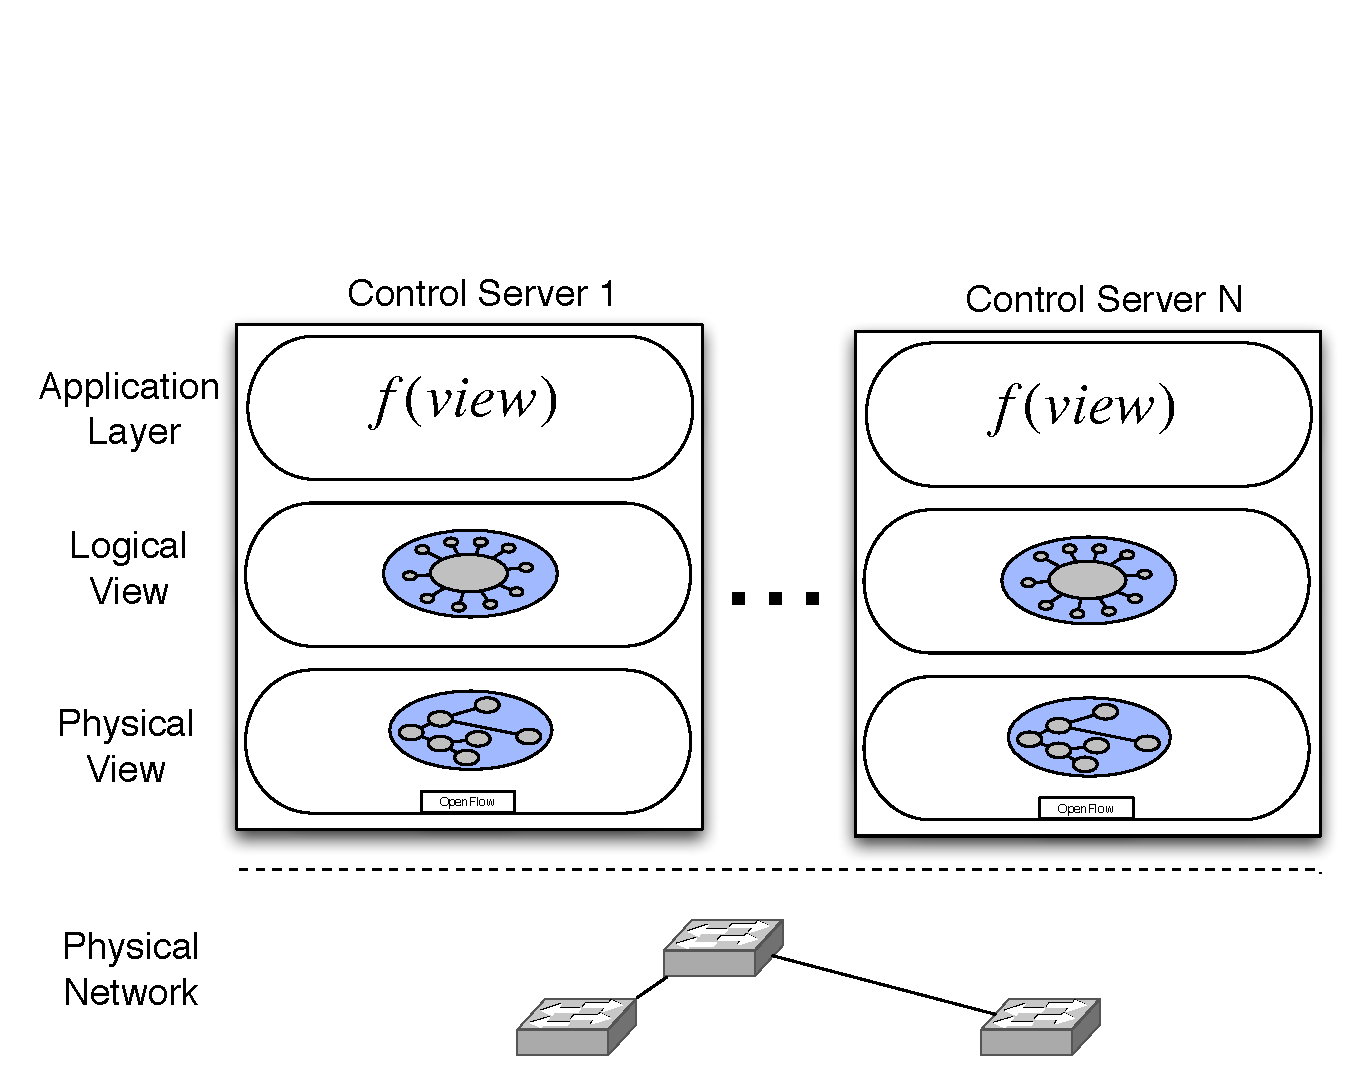
\includegraphics[width=3.25in]{../diagrams/architecture/SDN_Stack.pdf}
    \caption[]{\label{fig:basicarch} The SDN Software Architecture }
\end{figure}

Before describing the many ways in which such a system might fail, we note that there are two different kinds of SDN control applications: proactive and reactive.
Proactive applications pre-compute forwarding tables for the entire network,
and only push down updates periodically to react to link failures, changes in
traffic mix, \etc. In contrast, reactive control applications forward all new flows to
control servers. After a control decision is made, a flow entry is installed
in the ingress switch, and the packet is forwarded along.
Production SDN deployments are commonly proactive, primarily due to the large
scale of datacenter networks and the current capabilities of forwarding hardware.
We focus on proactive controllers for the remainder of this paper,
although our troubleshooting mechanisms are also applicable to reactive
applications. 

\subsection{Platform Failure Modes}

\projectname{} is designed to troubleshoot the SDN platform; here we discuss a few examples of platform failures.
As described above, modern SDN platforms differ from
`first-generation' controllers such as NOX~\cite{nox} in two dimensions:
they extend vertically by providing a virtualization layer on top of
which control logic resides, and they extend horizontally by
distributing state across multiple control servers. Platform errors arise from both of
these extensions.

\noindent{\bf Virtualization}. Virtualization errors result from a mismatch between the logical
view and the state of the physical network. When an entire datacenter
network (up to 10,000 switches) is abstracted into a single logical switch,
the mapping between the logical switch and the
physical topology is highly complex; for example, a simple configuration
change such as ``the path from $A$
 to $B$ should pass through $C$'' must be implemented as routing entries in a sequence
of switches in the physical network. This mapping is further complicated in a multi-tenant environment \cite{Casado:2010:VNF:1921151.1921162} where each tenant specifies
policies on their own logical switch. In such a case, each controller must deal with multiple tenants, and each tenant's policies must be coordinated among multiple controllers. Maintaining isolation
between tenants is critical; updates to the physical network must therefore be
performed in a consistent fashion to ensure that isolation breaches do not occur
for any in-flight packets, despite hardware failures and message delays. 

\noindent{\bf Controller Coordination} Policy changes
that span multiple shards of the physical view (shards being statically-defined
partitions of the physical network small enough to be managed by a single control
server) require coordination between controllers. Coordination between controllers
is prone to a plethora of well-known failure modes, such as inconsistent reads 
race conditions over message arrivals, and unintended consequences of failover
logic. Errors may also result
from non-disjoint partitioning schemes between controllers, or incorrect delegation of control for different
portions of the network.

The difficulty of implementing controller coordination correctly has been
noted by leaders in industry as well as academia. In a recent
keynote~\cite{urs_keynote}, Google's Urs H$\ddot{\mathrm{o}}$elzle noted that
``[controller coordination] is going to cause some agnst, and
justifiably, in the industry''

In this paper we focus on bugs in the virtualization and controller
coordination components of the SDN software stack. We are primarily concerned with corner-case scenarios such as
correlated hardware failures, which are
the hardest to test {\it a priori}. Corner-case scenarios, while rare, cannot be ignored because of the distributed nature and large scale of
production networks.
